\documentclass[11pt]{article}

\usepackage[a4paper,margin=2.5cm]{geometry}
\usepackage{amsmath,amssymb}
\usepackage{graphicx}
\usepackage{listings}
\usepackage{xcolor}
\usepackage{hyperref}
\usepackage{booktabs}
\usepackage{caption}

% ---------------------------------------------------------------
% Code listing style (used with \lstinputlisting{...} once the
% src/, include/, and validation/ folders are uploaded alongside
% this main.tex file in the Overleaf project)
% ---------------------------------------------------------------
\lstdefinestyle{cppstyle}{
    language=C++,
    basicstyle=\ttfamily\small,
    keywordstyle=\color{blue!70!black}\bfseries,
    commentstyle=\color{gray},
    stringstyle=\color{orange!70!black},
    numbers=left,
    numberstyle=\tiny\color{gray},
    stepnumber=1,
    breaklines=true,
    frame=single,
    showstringspaces=false,
    tabsize=4
}
\lstset{style=cppstyle}

\title{Non-Dominated Points (Maxima of a Point Set)\\
\large Progress Report}
\author{Arun Dinesh Jana \\ Matrikel-Nr.: 2227229 \\ Bergische Universit\"at Wuppertal}
\date{\today}

\begin{document}

\maketitle

\begin{abstract}
This report documents the progress made so far on the implementation and
experimental study of the \emph{maxima-of-a-point-set} problem (also known
as computing the \emph{non-dominated} or \emph{Pareto-optimal} points of a
set). A C++17 divide-and-conquer implementation of the \textsc{Maxima2}
algorithm and its \textsc{Filter}/\textsc{Filter2} merge subroutine has
been completed, following the classical treatment of the maxima problem by
Preparata and Shamos. The implementation has been validated against
hand-constructed test datasets and benchmarked empirically across varying
input sizes. This document summarizes the problem definition, algorithmic
approach, implementation structure, validation methodology, and the
benchmarking results obtained to date, and outlines the parallelization
work (MPI, CUDA) planned as the next stage of the project.
\end{abstract}

\tableofcontents

% =================================================================
\section{Problem Statement}
% =================================================================

Given a set $S$ of $N$ points in $E^d$ (i.e., $d$-dimensional Euclidean
space with integer coordinates), a point $p$ \emph{dominates} a point $q$
if $p$ is greater than or equal to $q$ in every coordinate, with strict
inequality in at least one coordinate:
\begin{equation}
p \succ q \iff \big(\forall i \in \{1,\dots,d\}: p_i \geq q_i\big)
\ \wedge\ \big(\exists i \in \{1,\dots,d\}: p_i > q_i\big).
\end{equation}
A point is a \emph{maximum} (equivalently, \emph{non-dominated} or
\emph{Pareto-optimal}) point of $S$ if no other point in $S$ dominates it.
The \emph{maxima problem} asks for the set of all such points. This is a
classical problem in computational geometry with applications in
multi-objective optimization, database skyline queries, and decision
theory.

% =================================================================
\section{Algorithmic Approach}
% =================================================================

The project implements the divide-and-conquer \textsc{Maxima2} algorithm
together with its recursive \textsc{Filter} merge step, as described in
Preparata and Shamos, \emph{Computational Geometry: An Introduction}.

\subsection{Dominance Relation}

The dominance predicate defined above is implemented directly as a
coordinate-wise comparison over the first $d$ coordinates of two points.

\lstinputlisting[caption={Dominance predicate}, label=lst:dominance]{src/dominance.cpp}

\subsection{\textsc{Maxima2}: Divide-and-Conquer Maxima}

The algorithm proceeds as follows:
\begin{enumerate}
    \item Sort the point set by its last coordinate.
    \item Split the sorted set at the median, adjusting the split point so
    that all points tied on the last coordinate fall on the same side
    (this preserves correctness of the recursive step).
    \item Recursively compute the maxima of the ``lower'' half $S_1$ and
    the ``upper'' half $S_2$, obtaining $M_1$ and $M_2$ respectively.
    \item \textbf{Merge}: every point of $M_2$ is automatically a maximum
    of $S$. A point of $M_1$ survives only if it is not dominated, on the
    remaining $d-1$ coordinates, by any point of $M_2$ --- this check is
    delegated to \textsc{Filter}.
    \item If the recursion bottoms out with all points tied on the last
    coordinate (i.e., the median split fails to separate the set), the
    maxima are computed directly by brute-force pairwise comparison.
\end{enumerate}

\lstinputlisting[caption={\textsc{Maxima2} divide-and-conquer driver}, label=lst:maxima2]{src/maxima2.cpp}

\subsection{\textsc{Filter} and \textsc{Filter2}: The Merge Step}

\textsc{Filter}$(U, V, d)$ computes the subset of $U$ that is not
dominated by any point of $V$, considering only the first $d$
coordinates. Because the coordinate that has been dropped from the
comparison already dominates strictly, a point of $V$ that merely ties
on the remaining coordinates still dominates: \textsc{Filter} uses weak
dominance there. The general recursive case works by:
\begin{itemize}
    \item Equipartitioning $V$ on coordinate $d$ into $V_1$ (lower half)
    and $V_2$ (upper half), via \textsc{PartitionV}.
    \item Deriving a splitting threshold from the maximum $d$-th
    coordinate in $V_1$, via \textsc{ThresholdFromV1}.
    \item Splitting $U$ at that threshold into $U_1$ and $U_2$, via
    \textsc{SplitU}.
    \item Recursing on three sub-problems --- $(U_2, V_2, d)$,
    $(U_1, V_1, d)$, and $(U_1, V_2, d-1)$ --- and recombining the
    results. The third sub-problem is applied to the survivors of the
    second, which computes the same intersection without materialising
    two intermediate sets.
\end{itemize}
The recursion bottoms out at $d = 1$ (a simple coordinate threshold
test) and at $d = 2$, where \textsc{Filter2} performs a linear-time
plane sweep over the remaining two coordinates.

\lstinputlisting[caption={\textsc{Filter} and \textsc{Filter2}}, label=lst:filter]{src/filter.cpp}

\lstinputlisting[caption={Equipartition of $V$}, label=lst:partition]{src/partition.cpp}

\lstinputlisting[caption={Threshold extraction from $V_1$}, label=lst:threshold]{src/threshold.cpp}

\lstinputlisting[caption={Threshold-based split of $U$}, label=lst:splitu]{src/split_u.cpp}


\lstinputlisting[caption={Coordinate-based sorting helpers}, label=lst:sorting]{src/sorting.cpp}

% =================================================================
\section{Implementation}
% =================================================================

The implementation is written in C++17 and organized as a small modular
library plus the benchmark and test programs built with CMake. Both
\textsc{Maxima2} and \textsc{Filter} operate in place on disjoint ranges
of one contiguous buffer: each recursive step partitions its range and
compacts its result to the front, so no level of the recursion copies its
input.

\subsection{Data Structures}

Points are represented by a simple aggregate:
\lstinputlisting[caption={Point representation}, label=lst:item]{include/item.hpp}

\subsection{Repository Structure}

\begin{verbatim}
non-dominated-points/
|-- src/
|   |-- main.cpp                 (MAXIMA2 benchmark driver)
|   |-- main_bruteforce.cpp      (brute-force benchmark driver)
|   |-- benchmark_runner.cpp     (shared loading and timing)
|   |-- benchmark.cpp            (CSV output)
|   |-- point_set.cpp            (dimension validation)
|   |-- dominance.cpp
|   |-- sorting.cpp
|   |-- maxima2.cpp
|   |-- brute_force_maxima.cpp
|   |-- filter.cpp
|   |-- partition.cpp
|   |-- split_u.cpp
|   |-- threshold.cpp
|   `-- print.cpp
|-- include/                     (corresponding headers)
|-- mpi_src/                     (ring, fan-in/fan-out, marry-go-round)
|-- DataSets/                    (benchmark inputs, 5D-10D)
|-- scripts/                     (dataset generator, sweep and job scripts)
|-- validation/
|   |-- validator.cpp
|   |-- validation_main.cpp
|   |-- differential_test.cpp
|   `-- test_datasets/           (Test1.txt .. Test16.txt)
|-- plots/
|   |-- plot_results.py
|   |-- plot_mpi_results.py
|   `-- figures/
|-- results/                     (generated benchmark CSVs)
`-- CMakeLists.txt
\end{verbatim}

\subsection{Random Data Generation}

Benchmark inputs are generated by drawing $n$ points with $D$
coordinates, each independently uniform on $[0,1]$ and rounded to six
decimals for storage, by a short Python script.

\lstinputlisting[language=Python,caption={Random point generation}, label=lst:gendata]{scripts/create_testcases.py}

\subsection{Build System}

The project is built with CMake and produces the MAXIMA2 and brute-force
benchmark drivers (\texttt{Maxima\_method}, \texttt{brute\_force}), the
\texttt{validator} and \texttt{differential\_test} test programs, and ---
when an MPI installation is available --- the three MPI programs
(\texttt{MPI\_Ringmethod}, \texttt{MPI\_FanInOut},
\texttt{MPI\_Marrygomethod}).

\lstinputlisting[language={},caption={CMakeLists.txt}, label=lst:cmake]{CMakeLists.txt}

% =================================================================
\section{Validation}
% =================================================================

Correctness of \textsc{Maxima2} is checked against 16 hand-constructed
test datasets stored in \texttt{validation/test\_datasets/}. Each dataset
file specifies the dimension, the input point set, and the expected set
of maxima, e.g.:

\begin{verbatim}
# Dimension
2

# Number of Input Points
1

# Input Points
5 5

# Number of Expected Maxima
1

# Expected Maxima
5 5
\end{verbatim}

The dataset loader parses this format and returns the input points
alongside the expected output for comparison.

\lstinputlisting[caption={Test dataset loader}, label=lst:validator]{validation/validator.cpp}

\lstinputlisting[caption={Header for validation types}, label=lst:validatorhpp]{include/validator.hpp}

The validation driver runs \textsc{Maxima2} on all 16 test cases and
reports a pass/fail summary, printing the expected and computed maxima
side by side whenever a mismatch occurs. Expected maxima are compared as
an unordered set, since the order in which maxima are listed carries no
meaning.

\lstinputlisting[caption={Validation driver}, label=lst:validationmain]{validation/validation_main.cpp}

\noindent In addition to these hand-built cases, \texttt{differential\_test}
compares \textsc{Maxima2} against the brute-force reference over 13\,104
generated cases (dimensions 2--8, point counts 2--40, integer and
fractional coordinate ranges chosen to produce ties and duplicate
points) with a fixed seed, so that a failure is reproducible. It also
checks that inconsistent point sets are rejected instead of being read
out of bounds. Both programs run under CTest.

\noindent At the current stage, all 16 test cases pass and the
differential test reports no mismatches.

% =================================================================
\section{Benchmarking}
% =================================================================

\subsection{Methodology}

The benchmark drivers load the datasets in \texttt{DataSets/} and measure
the wall-clock execution time of \textsc{Maxima2} and of the brute-force
baseline with \texttt{std::chrono::steady\_clock}, taking the median of 10
repetitions per configuration. Both drivers cover the same inputs,
\texttt{Test1} through \texttt{Test6} (50 to 100\,000 points); each
configuration occupies exactly one row, so re-running a dimension replaces
its measurements rather than duplicating them. Results are written to
\texttt{results/maxima\_benchmark.csv} and
\texttt{results/brute\_force\_benchmark.csv} and subsequently plotted by
\texttt{plots/plot\_results.py} (using pandas and matplotlib) into
\texttt{plots/figures/}.

\lstinputlisting[caption={Benchmark driver}, label=lst:main]{src/main.cpp}

\lstinputlisting[language=Python,caption={Plotting script}, label=lst:plot]{plots/plot_results.py}

\subsection{Results So Far}

To date, benchmarks have been run for a single fixed dimension,
$D = 10$, over input sizes ranging from $N = 100$ to $N = 100{,}000$
points. The raw measurements are reproduced in Table~\ref{tab:benchmark}.

\begin{table}[h]
\centering
\caption{Execution time of \textsc{Maxima2} for $D=10$ from an earlier
measurement run; the table is retained as a record and is regenerated by
the current benchmark driver.}
\label{tab:benchmark}
\begin{tabular}{rr}
\toprule
$N$ (points) & Execution time ($\mu$s) \\
\midrule
100     & 11{,}692.4 \\
500     & 70{,}702.9 \\
1{,}000   & 193{,}519 \\
5{,}000   & 1{,}873{,}410 \\
10{,}000  & 4{,}995{,}070 \\
50{,}000  & 37{,}591{,}500 \\
100{,}000 & 79{,}678{,}700 \\
\bottomrule
\end{tabular}
\end{table}

\begin{figure}[h]
\centering
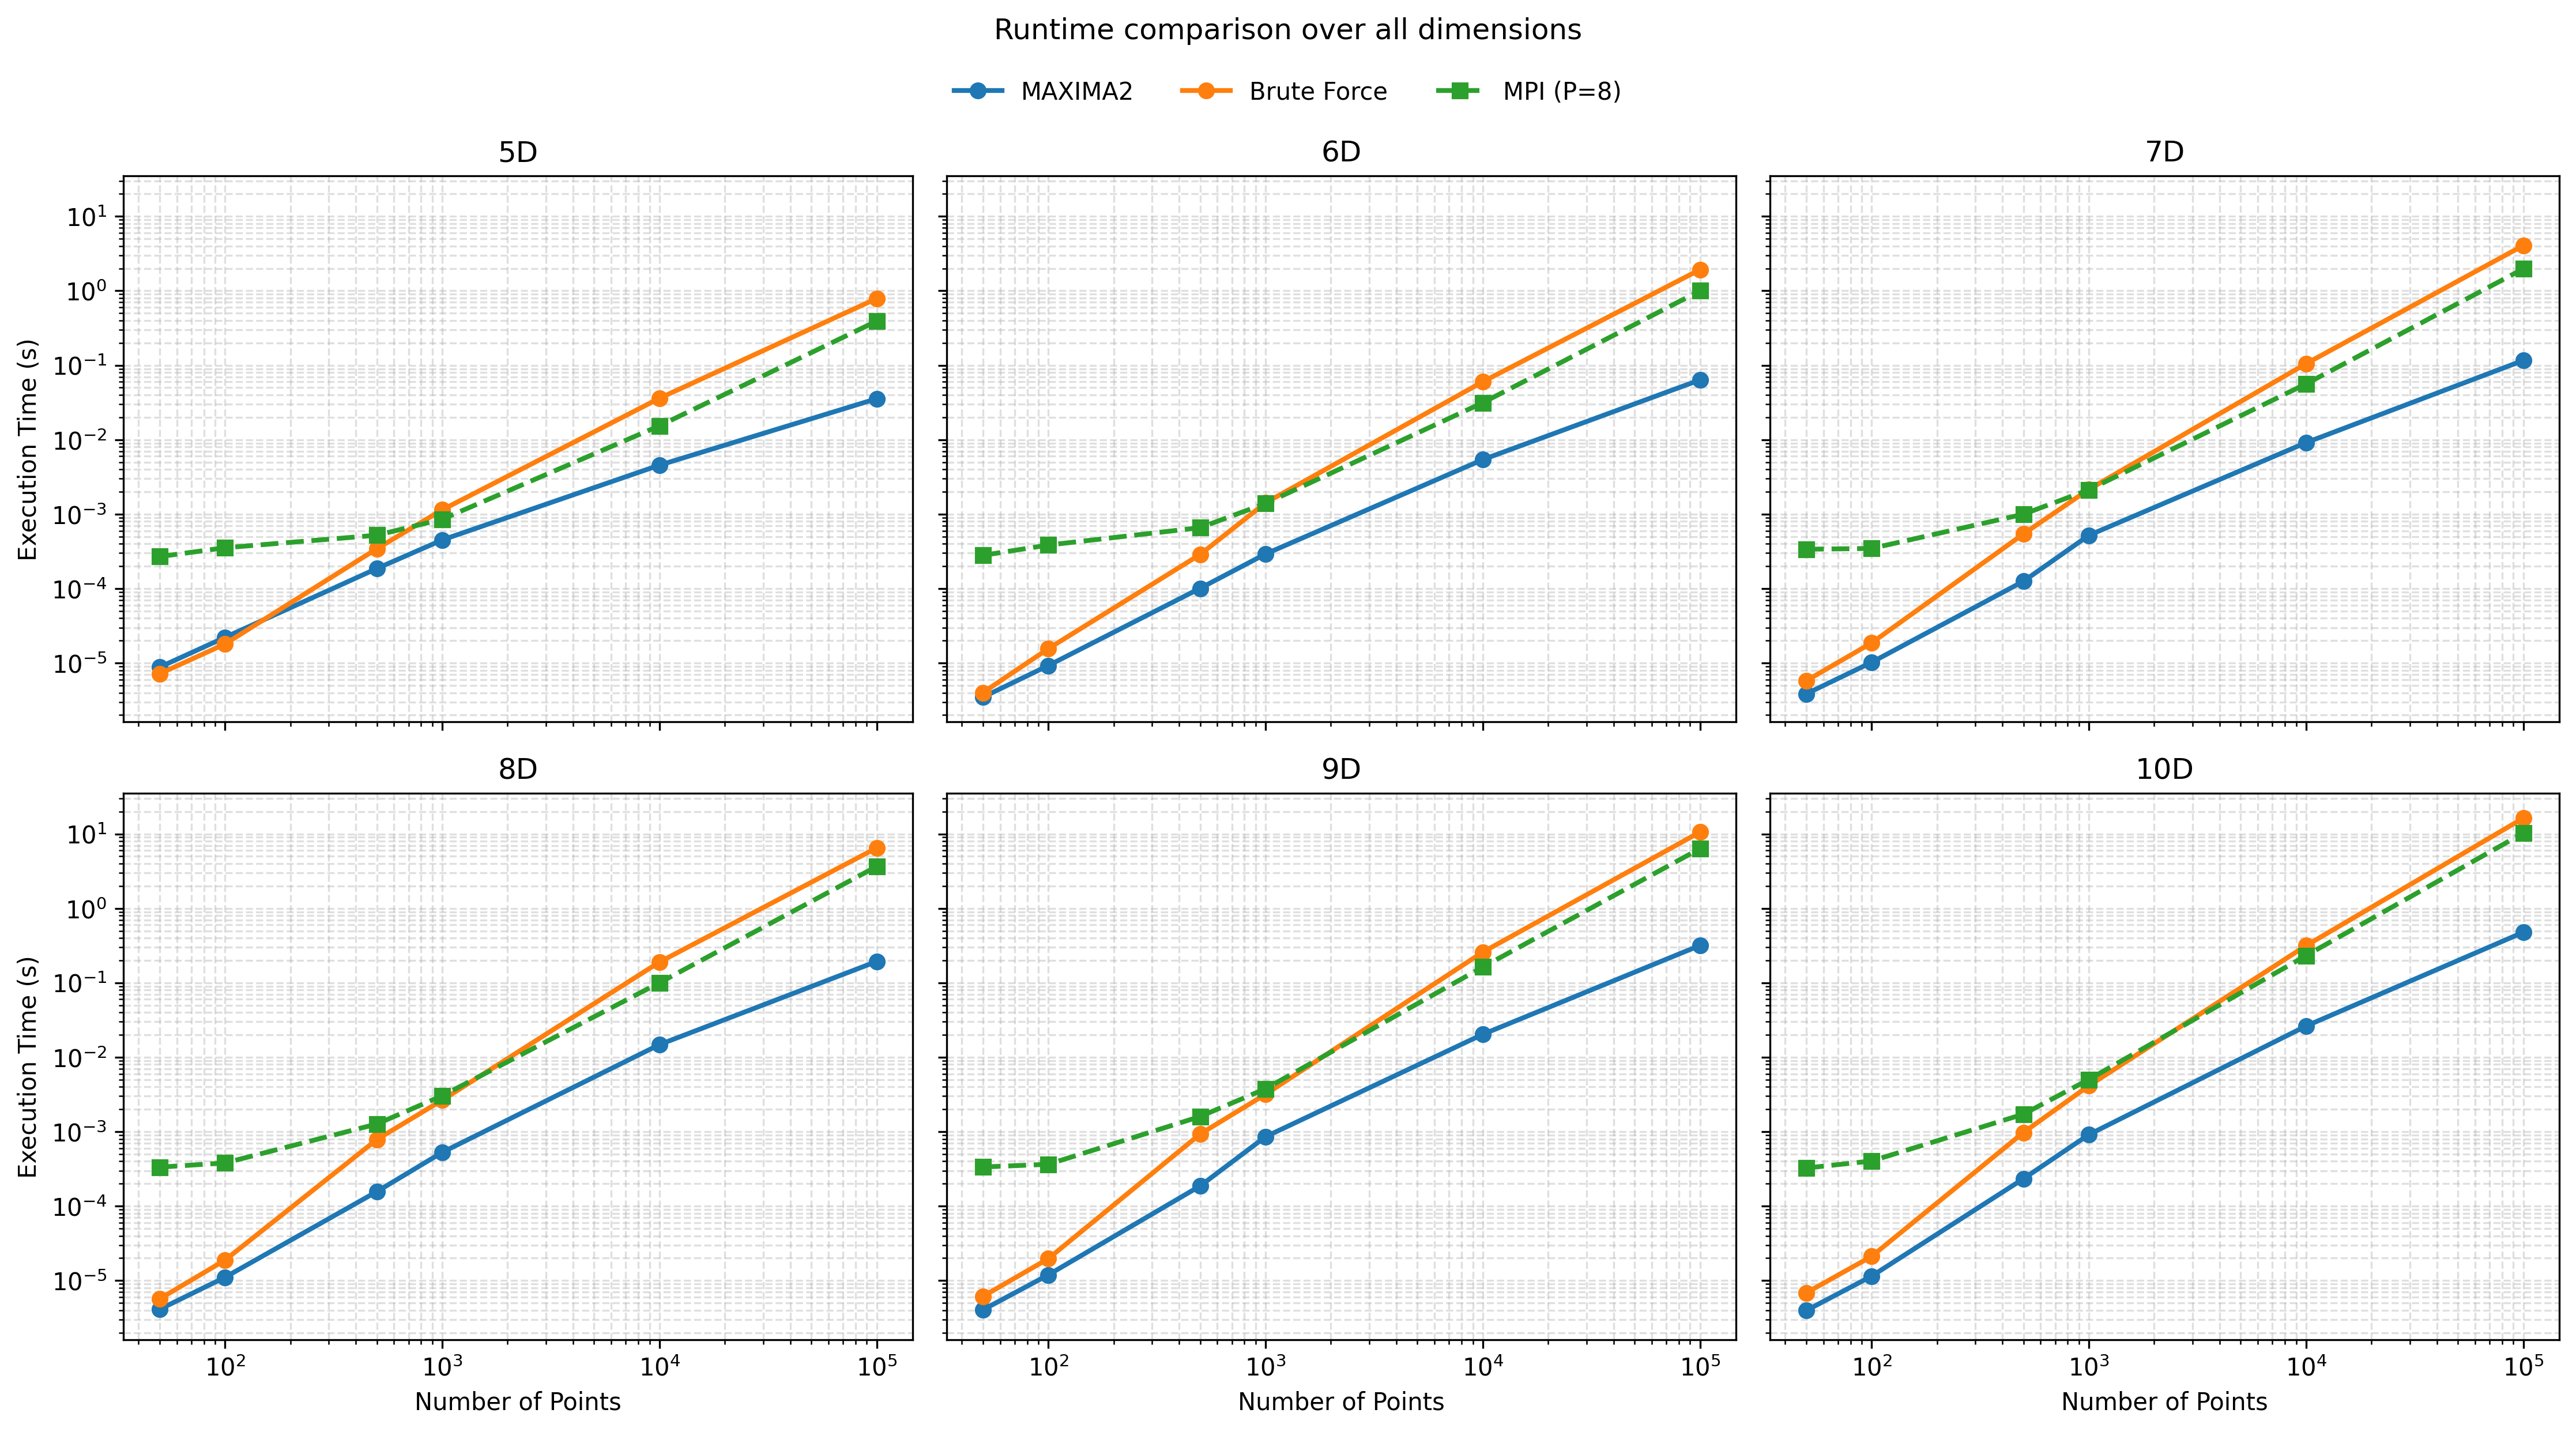
\includegraphics[width=0.9\textwidth]{plots/figures/runtime_comparison.png}
\caption{Execution time of \textsc{Maxima2} versus number of points, for
$D = 10$ (log-log scale).}
\label{fig:runtime10d}
\end{figure}

% TODO: discuss the observed growth rate versus the theoretical
% O(N log^{d-2} N) bound for MAXIMA2/FILTER once benchmarks across
% multiple dimensions (D = 2..10, as sketched in main.cpp) are available.

\subsection{Benchmarking Across Dimensions}

Each driver takes a dimension folder and covers the full series of input
sizes for that dimension, so runtime can be compared across both $N$ and
$d$. Generated inputs are available for five through ten dimensions;
smaller dimensions can be produced with the generator script if needed.

% =================================================================
\section{Progress Summary}
% =================================================================

\begin{itemize}
    \item \textbf{Completed:} dominance relation, random data generation,
    \textsc{Maxima2} divide-and-conquer driver (with brute-force
    fallback), full recursive \textsc{Filter}/\textsc{Filter2} merge
    step, an in-place range-based implementation of both algorithms, a
    validating point-set interface, CMake build system with the
    benchmark drivers, two test programs and three MPI programs,
    correctness validation against 16 hand-crafted test cases plus a
    randomized differential test, and a benchmarking pipeline with
    automated plot generation.
    \item \textbf{In progress / next steps:} run the benchmark suite over
    the full range of dimensions and compare the measured scaling with
    the theoretical bound.
\end{itemize}

% =================================================================
\section{Future Scope}
% =================================================================

The following extensions are planned for the next phase of the project:

\begin{itemize}
    \item \textbf{MPI (OpenMPI) implementation} --- three distributed
    strategies (ring, fan-in/fan-out, marry-go-round) have been
    implemented for the pairwise formulation. Distributing the
    divide-and-conquer recursion of \textsc{Maxima2}/\textsc{Filter}
    itself remains open, with particular attention to load-balanced merge
    steps.
    \item \textbf{CUDA implementation} --- parallelizing the dominance
    checks and the sweep/merge steps on the GPU for large point sets.
    \item \textbf{Performance evaluation} --- measuring speedup and
    scale-up of the parallel (MPI/CUDA) versions relative to the
    sequential baseline, across varying number of points $N$, dimension
    $d$, and number of processes/threads/GPU cores, and comparing strong
    versus weak scaling behavior for both parallelization strategies.
\end{itemize}

\end{document}